\documentclass{article}
\usepackage[utf8]{inputenc}

\title{Chem132A: Midterm 2 Solutions}
\author{Moises Romero, Shane Flynn}
\date{November 2017}


\usepackage{graphicx}
\usepackage{amsmath}
\usepackage{braket}
\usepackage[margin=0.7in]{geometry}
\usepackage[version=4]{mhchem}


\newcommand{\be}{\begin{equation}}
\newcommand{\ee}{\end{equation}}
\newcommand{\pd}{\partial}

\begin{document}

\maketitle


\section{Definitions \qquad (10 Points)}

\subsection{Intensive/Extensive}
For each of the following indicate if it is an \textbf{Intensive} or \textbf{Extensive} property.

\subsubsection*{Solution:}
\begin{tabular}{ l | c }
    Volume & Extensive\\
    Mass & Extensive\\
    Entropy & Extensive\\
    Density & Intensive\\
    Internal Energy & Extensive\\
    Pressure & Intensive\\
    Temperature & Intensive\\
    Gibbs Free energy & Extensive\\
    Helmholtz Free Energy & Extensive\\
    C$_P$ & Extensive\\
\end{tabular}

\subsection{Transport Properties \qquad (5 Points)}
Which gas has a higher thermal conductivity, He or Ar?		
Briefly explain	why.

\subsubsection*{Solution:}
Thermal Conductivity considers the flux of thermal energy (thermal motion).
Both Argon and Helium can be approximated as spheres (no quantum effects, no structure to store excess energy) therefore the only difference between the two is mass.
Helium has a much smaller mass than Argon, it must have a higher mean speed, and a subsequently higher thermal conductivity. 

\subsection{Boltzmann Speed Distribution}
\begin{figure}[h]
\centering
\caption{The figure below shows the Boltzmann speed distribution f(v) for a	 gas.
CLEARLY label on the figure the v$_{mp}$, v$_{mean}$, and v$_{rms}$.}
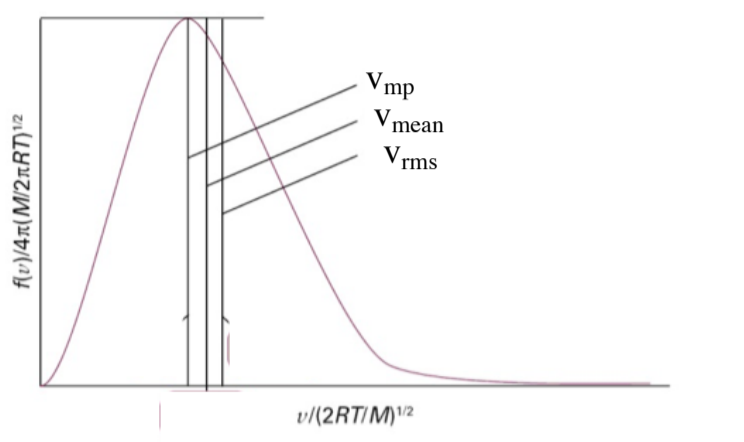
\includegraphics[width=0.47\textwidth]{midterm2_1.png}
\end{figure}

\section{Non-Ideal Liquid Mixture \qquad (30 Points)}
Consider the mixing of two non-ideal liquids; species 1 and species 2 respectively. 

\subsection{Assumptions}
Because our system is no longer ideal, what are the two most important assumptions we can no-longer make about the mixing process?

\subsubsection*{Solution:}
The two huge assumptions for physical mixing are
\be
\Delta_{mix}H = 0
\ee
And
\be
\Delta_{mix}V_m = 0
\ee
With a non-ideal solution we should not expect either of these statements to be true, and we will show this for the Enthalpy later on.

\textbf{Comment:} Raoult's Law is not relevant to the physical mixing process itself, it simply relates the vapour phases of an ideal mixture. 

\subsection{Gibbs Free Energy}
Analogous to the Ideal Mixing Equation, we should define the Gibbs Free Energy of a non-ideal solution to be 
\be
\Delta_{mix}G = nRT\left[x_1\ln(a_1) + x_2\ln(a_2)\right]
\ee
Starting from this equation, show that 
\be
\Delta_{mix}G = nRT\left[x_1\ln(x_1) + x_2\ln(x_2) + \beta x_1x_2\right]
\ee

\textbf{Assume:}
\begin{itemize}
\item $\ln(\gamma_1) = \beta x_2^2$
\item $\ln(\gamma_2) = \beta x_1^2$
\end{itemize}

\subsubsection*{Solution:}
We start with the general definition of the activity.
\be
a_i = \gamma_i x_i
\ee
We need to then substitute in this relationship, and work through the math.
\be
\begin{split}
\Delta_{mix}G &= nRT\left[x_1\ln(\gamma_1x_1) + x_2\ln(\gamma_2x_2)\right]\\
&= nRT\left[x_1\ln(x_1) + x_1\ln(\gamma_1) + x_2\ln(x_2) + x_2\ln(\gamma_2)\right]
\end{split}
\ee
We can now substitute in our assumptions for the activity coefficients.
\be
\begin{split}
\Delta_{mix}G &= nRT\left[x_1\ln(x_1) + x_2\ln(x_2) + x_1\beta x_2^2 + x_2\beta x_1^2\right]\\
&= nRT\left[x_1\ln(x_1) + x_2\ln(x_2) + \beta x_1x_2(x_2+x_1)\right] \\
\Delta_{mix}G &= nRT\left[x_1\ln(x_1) + x_2\ln(x_2) + \beta x_1x_2\right]
\end{split}
\ee
Where the last line follows from the fact that the two mole fractions must add up to one for a binary mixture. 

\subsection{Fundamental Equation}
Starting from the Fundamental Equation for the Gibbs Free Energy, determine the appropriate derivative for Entropy (assume constant pressure).

\subsection*{Solution:}
We start by writing down the Fundamental Equation for the Gibbs Free Energy.
\be
dG = VdP - SdT + \sum_i \mu_i dn_i 
\ee
This is a simple mixing problem (no chemical reactions) and the system is assumed to be closed.
Therefore dn = 0. 
Likewise we are told the pressure is constant therefore dP = 0. 
\be
dG = -SdT \rightarrow S = -\left(\frac{\pd G}{\pd T}\right)_{P,n_i}
\ee

\subsection{Computing Non-Ideal Entropy}
Assuming the variable $\beta$ is linearly proportional to temperature (i.e. $\beta=cT$) where c is a constant, compute the Entropy of Mixing. 

\subsubsection*{Solution:}
Because we assume $\beta$ is linearly proportional to T we simply take the derivative.
\be
\begin{split}
S &= -\left(\frac{\pd G}{\pd T}\right)_{P,n_i}\\
\Delta_{mix}S &= - \left(\frac{\pd \Delta_{mix}G}{\pd T}\right)_{P,n_i}\\
&= - \frac{\pd}{\pd T} nRT\left[x_1\ln(x_1) + x_2\ln(x_2) + \beta x_1x_2\right] \\
&= -nR\left[x_1\ln(x_1) + x_2\ln(x_2) + x_1x_2\frac{\pd}{\pd T}T\beta \right]\\
\Delta_{mix}S &= -nR\left[x_1\ln(x_1) + x_2\ln(x_2) + 2cTx_1x_2 \right]
\end{split}
\ee

\subsection{Enthalpy}
From the definition of the Gibbs Free Energy, compute the Enthalpy of Mixing (assume there is no change in temperature due to mixing). 

\subsubsection*{Solution}
From the definition of the Gibbs Thermodynamic Potential we know that
\be
\begin{split}
G &= H - TS\\
\Delta_{mix}G &= \Delta_{mix}H - T\Delta_{mix}S\\
\Delta_{mix}H &= \Delta_{mix}G + T\Delta_{mix}S\\
&= nRT\left[x_1\ln(x_1) + x_2\ln(x_2) + \beta x_1x_2\right] + -nRT\left[x_1\ln(x_1) + x_2\ln(x_2) + 2cTx_1x_2 \right]\\
\Delta_{mix}H &= -nRT\beta x_1x_2
\end{split}
\ee
The last line follows from:
\be
\begin{split}
nRT\beta x_1x_2 - nRT2cTx_1x_2 \rightarrow\\
nRT\beta x_1x_2 - nRT2\beta x_1x_2 \rightarrow \\
nRT\beta x_1x_2(1-2) \rightarrow \\
-nRT\beta x_1x_2 = -cnRT^2x_1x_2
\end{split}
\ee

\newpage

\section{Reaction Quotient}
Consider the reaction for methanol : 
\be
2H_2(g) + CO(g) \rightarrow CH_3OH(g) 
\ee

\subsection{Calculating Standard Gibbs Free Energy}
Standard Gibbs values for the compounds are as follows : 

\bigskip
$\Delta_fG^o (kJmol^{-1}) CH_3OH(g) = $ -161.96

\bigskip

$\Delta_fG^o (kJmol^{-1}) CO(g) =$ -137.17

\bigskip

$\Delta_fG^o (kJmol^{-1}) H_2(g) =$ 0

\bigskip
Calculate ($\Delta_{rxn}G^o$) the standard Gibbs Free Energy of the reaction. 

\subsubsection*{Solution:}
We know that we simply take the cost to generate the products minus the energy associated with the reactants. 
\be
(\Delta_{rxn}G^o) = -161.96 - [-137.17+0] = -24\text{kJmol$^{-1}$}
\ee

\subsection{Calculating K}
Calculate K$_P$ for the reaction at 298K. 

\subsubsection*{Solution:}
Using the Gibbs Free Energy (at standard conditions) we can calculate K (at constant pressure)
\be
\begin{split}
\Delta_rG &= \Delta_rG^0 + RT \ln Q \\
\xrightarrow{\text{equ}} &= \Delta_rG^0 = -RT \ln K\\
K &= e^{\frac{-\Delta_{rxn}G^o}{RT}} = e^{\frac{24}{(.008314)(298)}} = 2.21 \times 10^{4} 
\end{split}
\ee

\subsection{Calculating Q}
For the following pressures : $P_{CH_3OH}$ = 10 Bar , $P_{CO}$ = .005 Bar , $P_{H_2}$ = .10 Bar , write the expression for and calculate Q. 
Based on the calculated Q and K$_P$, in what direction will the reaction proceed to reach equilibrium? 

\subsubsection*{Solution:}
Assuming we can write Q as a function of Pressure only (since we only have information about pressure) and taking our reference terms to all be 1 Bar.
\be
Q =\frac{P_{CH_3OH}}{(P_{CO})(P_{H_2})^2} = \frac{10}{(.005)(.1)^2} = 2 \times 10^5 
\ee

Q$>$K; $\qquad$ therefore the reaction will proceed to the left to reach equilibrium.
It favors the reactants.
\bigskip

\subsection{Calculating Gibbs Free Energy}
Calculate the Gibbs free energy for the calculated Q.

\subsubsection*{Solution:}
Again using our expression for the Gibbs Free Energy we find:
\be
\Delta_rG = \Delta_rG^o +RTlnQ = -24 + (.008314)(298)\ln(2 \times 10^5 ) = 6.24\text{kJmol$^{-1}$}
\ee
\bigskip

\subsection{Relationship Between Equilibrium Constants}
What is the relationship between K$_P$ , K$_{\gamma}$, and K$_f$?

\subsubsection*{Solution:}
Just as presented in the Discussion Homework, we can write down an equilibrium constant in terms of fugacity, pressure, and activity. 

For a general reaction :
\be 
aA + bB \rightarrow cC + dD
\ee
We know that the fugacity is directly related to the fugacity coefficient. 
\be
K_f = \frac{{f^{(c)}_Cf^{(d)}_D}}{{f^{(a)}_Af^{(b)}_B}} = \frac{{\gamma^{(c)}_PP^{(c)}_C\gamma^{(d)}_DP^{(d)}_D}}{{\gamma^{(a)}_AP^{(a)}_A\gamma^{(b)}_B}P^{(b)}_B} = \left(\frac{\gamma^{(c)}_C\gamma^{(d)}_D}{\gamma^{(a)}_A\gamma^{(b)}_B}\right)
\left(\frac{P^{(c)}_CP^{(d)}_D}{P^{(a)}_AP^{(b)}_B}\right) = K_\gamma \dot K_P
\ee

\bigskip
Under what conditions does  K$_P$ approximately equal K$_f$ and why?

The most direct statements is at low pressures.
At low pressures we know that gases behave ideally, and we do not need correction terms 
(i.e. the activity coefficient; $K_\gamma$ $\rightarrow$ 1). 

\newpage

\section{Ionic Solutions}
The \textbf{Debye-Huckel Limiting Law} is given by
\be
\log \gamma_\pm = -0.509|z_+z_-|\sqrt{I}
\ee

\subsection{KCl}
Calculate the mean activity coefficient of a solution that is 5.0 mmol/kg of KCl in water at 25$^0$C. 
KCl is a very soluble salt. 

\subsubsection*{Solution:}
If we take the reference concentration to be 1 we can write
\be
\begin{split}
I &= \frac{1}{2}\sum_i b_i z_i^2\\
&= \frac{1}{2} \left[(0.005)(1)^2 + 0.005*(-1)^2\right]\\
I &= 0.005
\end{split}
\ee
Now we can solve for the log of the activity coefficient. 
\be
\begin{split}
\log \gamma_\pm &=  -0.509|1*-1|\sqrt{0.005} \\
\log \gamma_\pm &\approx -0.0359917 \\
\gamma_\pm &\approx 0.92
\end{split}
\ee

\subsection{CaCl$_2$}
Calculate the mean activity coefficient of a solution that is 1.0 mmol/kg of CaCl$_2$ in water at 25$^0$C. 
CaCl$_2$ is a very soluble salt. 

\subsubsection*{Solution:} 
This question is very similar, remember to account for the two negative ions that are generated upon dissociation. 
\be
\begin{split}
I &= \frac{1}{2}\sum_i b_i z_i^2\\
&= \frac{1}{2} \left[(0.001)(2)^2 + 2*0.001*(-1)^2\right]\\
I &= 0.003
\end{split}
\ee
Now we can solve for the log of the activity coefficient. 
\be
\begin{split}
\log \gamma_\pm &=  -0.509|2*-1|\sqrt{0.003} \\
\gamma_\pm &\approx 0.88
\end{split}
\ee

\subsection{Explain}
If you did the calculations in question 4.1 and 4.2 correct you would see that the 5.0 mmol/kg KCl solution is more ideal than the 1.0 mmol/kg CaCl$_2$ solution, even though the KCl solution is more concentrated.  
What is the simple explanation for this

\subsection*{Solution}
The most important factor is the positive 2 charge of the calcium ion. 
Remember the Coulomb Force is a long-distance force (its value approaches 0 slowly), therefore charges propagate throughout your system.

This is accounted for in the Ionic Strength by squaring the charges. 

It is important to also note that the calcium chloride puts three ions into solution upon dissociation not two further complicating the scenario when compared to a simple salt like KCl. 

\end{document}